In this section, we discuss the performance of \pred\ when the number of actions is very high so that the weak demonstrator $\pi^w$ does not have sufficient samples for each action. However, the number of tasks $\Mpr \gg A > n$.

\textbf{Baselines:} We again implement the same baselines discussed in \Cref{sec:short-horizon}. The baselines are \pred, \predt, \dptg, \ad, \ts, and \linucb. 


\textbf{Outcomes:} We first discuss the main outcomes from our experimental results of introducing more actions than the horizon (or more dimensions than actions) during data collection and evaluation:

\begin{tcolorbox}
\customfinding \pred\ (\gt) outperforms \dptg, and \ad, even when $A > n$ but $\Mpr \gg A$.
\end{tcolorbox}

% \noindent
% \textbf{(1)} The \pred\ (\gt) exploits the underlying latent structure and reward correlation between the different tasks even when $A > n$ but $\Mpr \gg A$.

% \textbf{(2)} The \pred\ (\gt) has lower regret than its weak demonstrator even when it is trained on $\Htr\subseteq\Dpr$.

% \textbf{(3)} The \pred\ (\gt) performance drops for complex non-linear bandit setting with increasing number of dimensions.





% \begin{figure}[!hbt]
% \centering
% \vspace*{-1.5em}
% \begin{tabular}{cc}
% \subfigure[Linear Bandit]{\hspace*{-1.5em}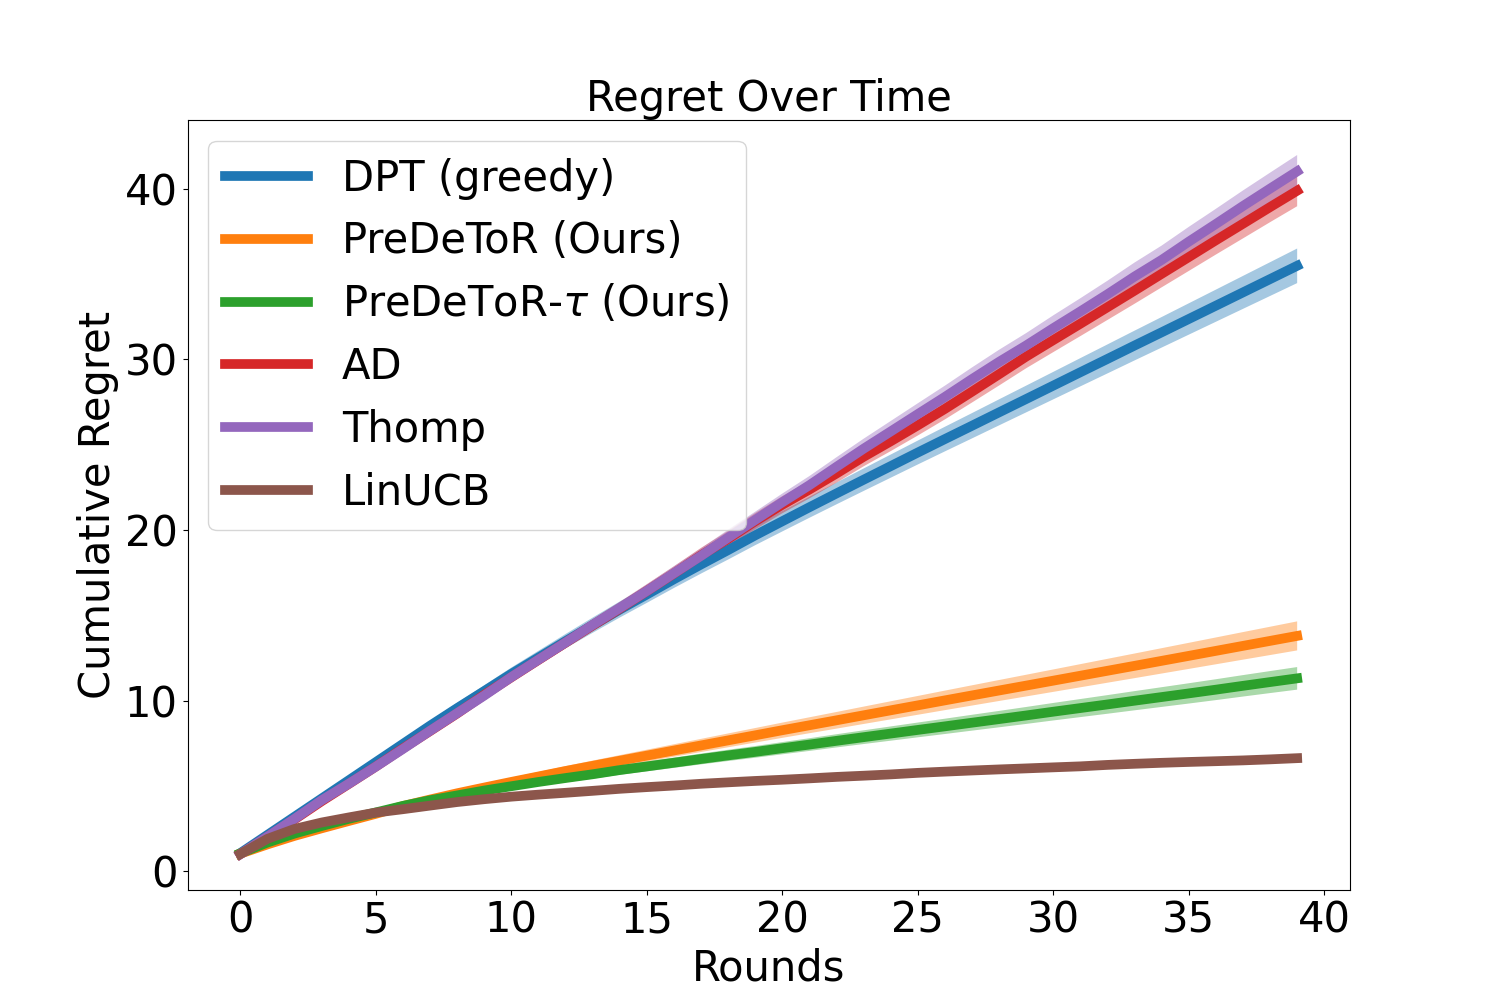
\includegraphics[scale = 0.15]{img/Neurips/limit/lin_lim_lr0.00015_do0_embd32_layer4_head4_envs200045_hists1_samples1_var0.3_cov0.0_H40_d100_lind5_seed1_testcov0.0_hor40.pkl.png}\label{fig:lim-lin}} &
% %%%%%%%%%%
% \hspace*{-1.5em}\subfigure[Non-linear Bandit]{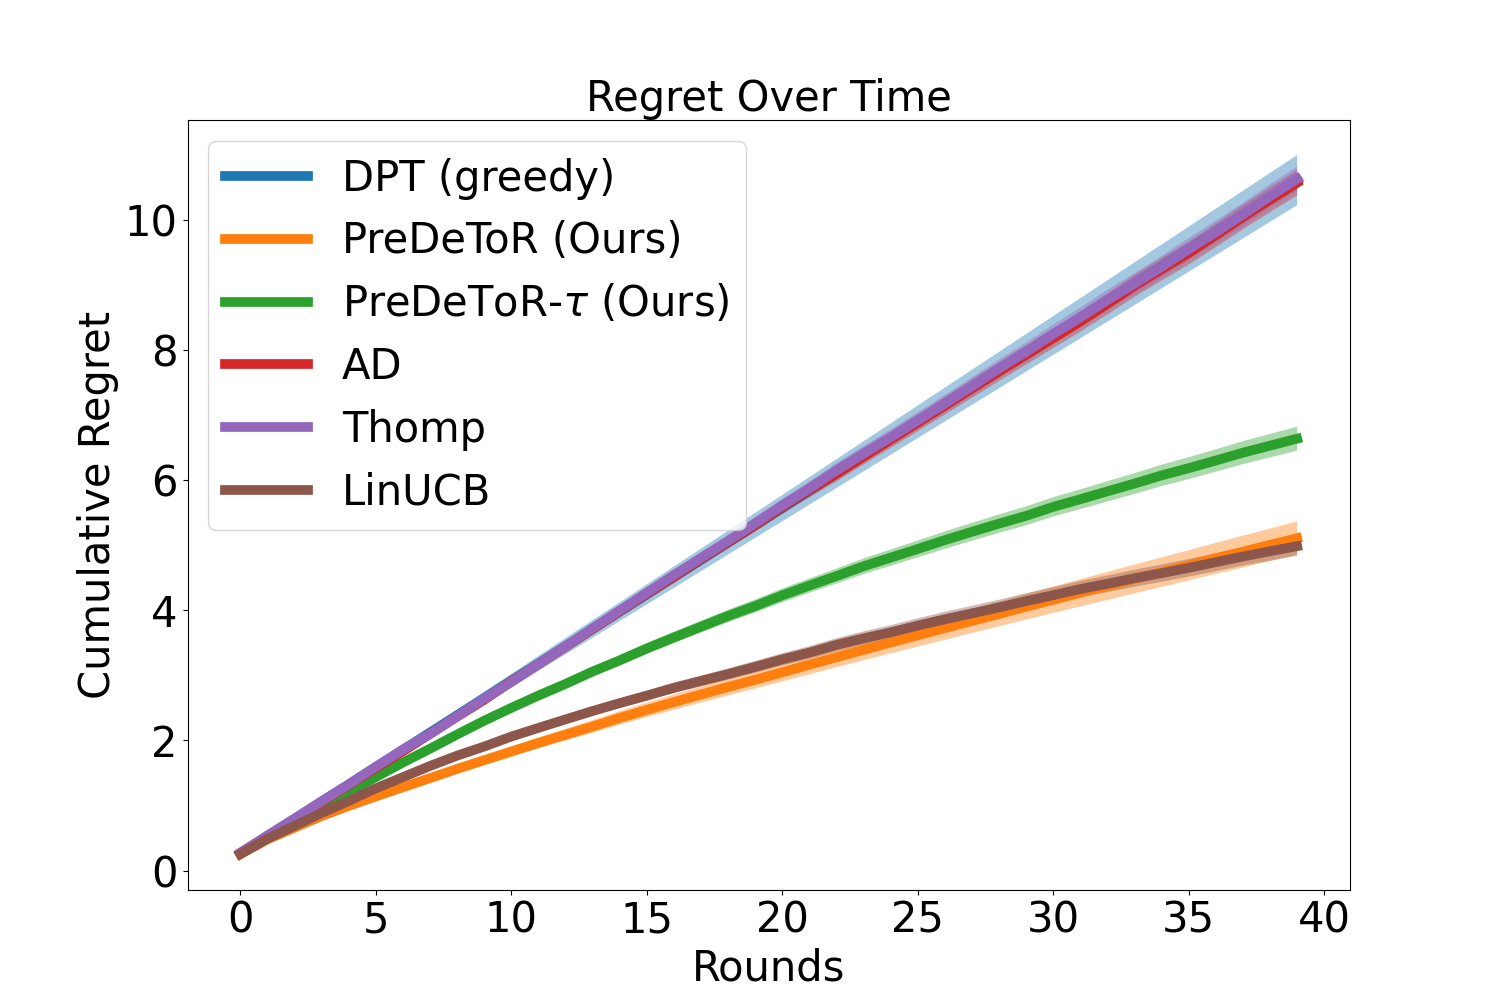
\includegraphics[scale = 0.15]{img/Neurips/limit/nlm_lim_lr0.00015_do0_embd32_layer4_head4_envs200195_hists1_samples1_var0.3_cov0.0_H40_d100_lind5_seed1_testcov0.0_hor40.pkl.png} \label{fig:lim-nlm}}%\\
% %%%%%%%%%%%%%%%%%%%%%%%
% % \subfigure[Linear Bandit]{\hspace*{-1.5em}\includegraphics[scale = 0.1]{img/final/limit/dims/lin_dim_lr0.00015_do0_embd32_layer4_head4_envs400000_hists1_samples1_var0.3_cov0.0_H20_d20_lind40_seed1_testcov0.0_hor20.pkl.png}\label{fig:lim-dim-lin}} &
% % %%%%%%%%%%
% % \hspace*{-1.5em}\subfigure[Non-linear Bandit]{\includegraphics[scale = 0.1]{img/final/limit/dims/nlm_dim_lr0.00015_do0_embd32_layer4_head4_envs400000_hists1_samples1_var0.3_cov0.0_H20_d20_lind40_seed1_testcov0.0_hor20.pkl.png} \label{fig:lim-dim-nlm}}
% \end{tabular}
% \vspace*{-1em}
% \caption{Testing the limit experiments. The horizontal axis is the number of rounds. Confidence bars show one standard error.}
% \label{fig:expt-lim}
% \vspace{-0.7em}
% \end{figure}

\begin{figure}[!hbt]
\centering
% \vspace*{-1.5em}
\begin{subfigure}[b]{0.48\textwidth}
   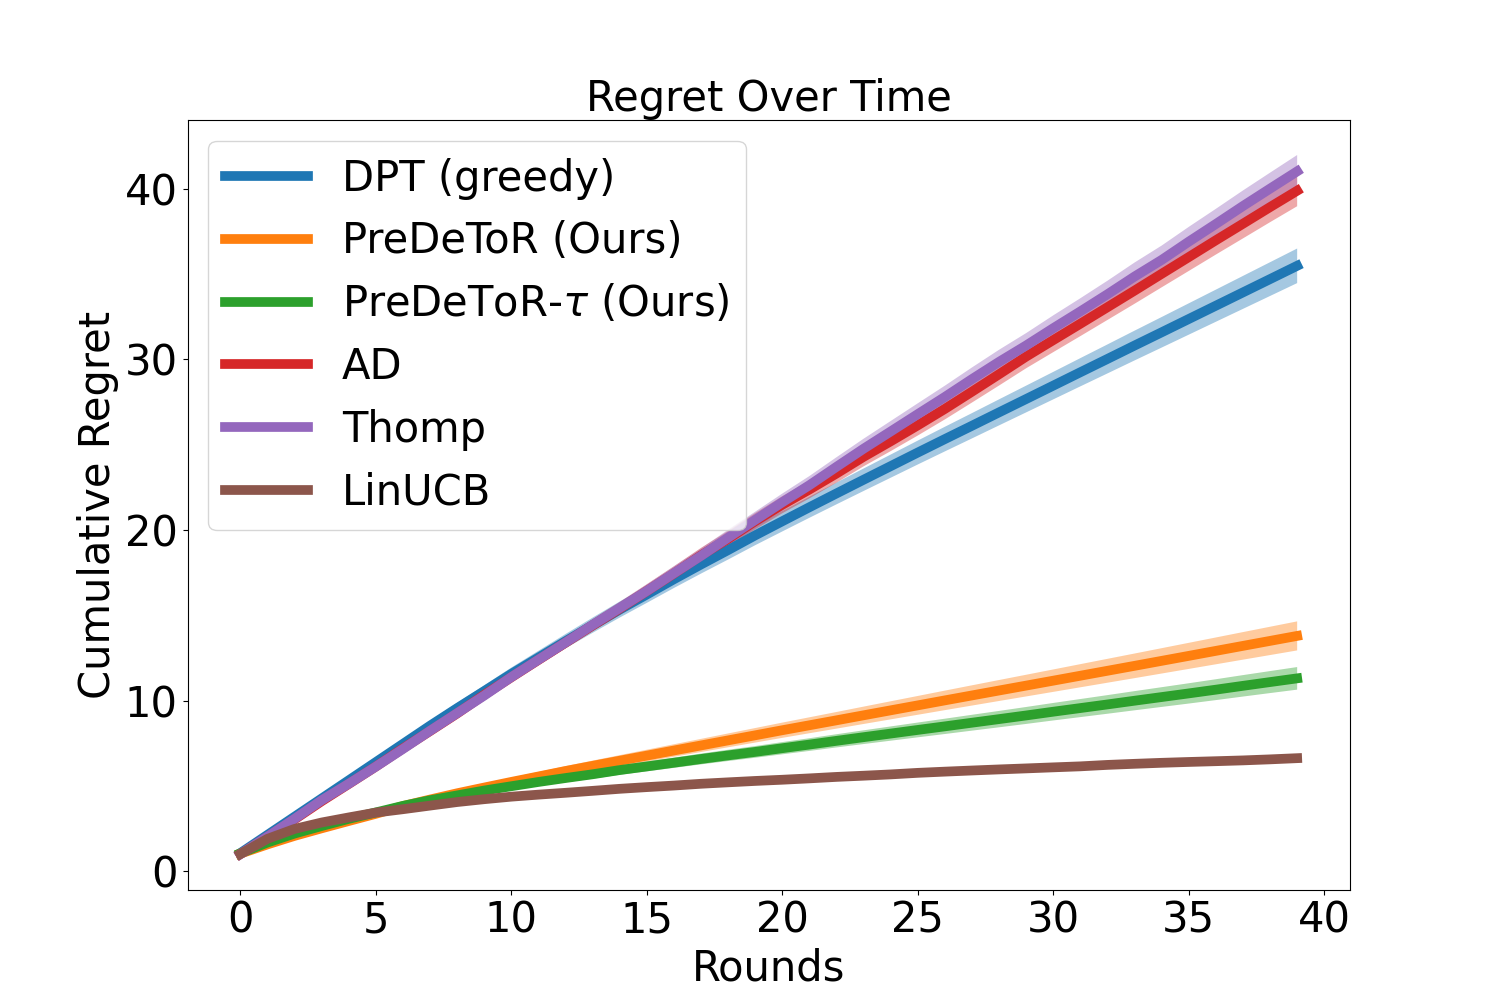
\includegraphics[scale=0.15]{img/Neurips/limit/lin_lim_lr0.00015_do0_embd32_layer4_head4_envs200045_hists1_samples1_var0.3_cov0.0_H40_d100_lind5_seed1_testcov0.0_hor40.pkl.png}
   \caption{Linear Bandit}
   \label{fig:lim-lin}
\end{subfigure}%
\begin{subfigure}[b]{0.48\textwidth}
   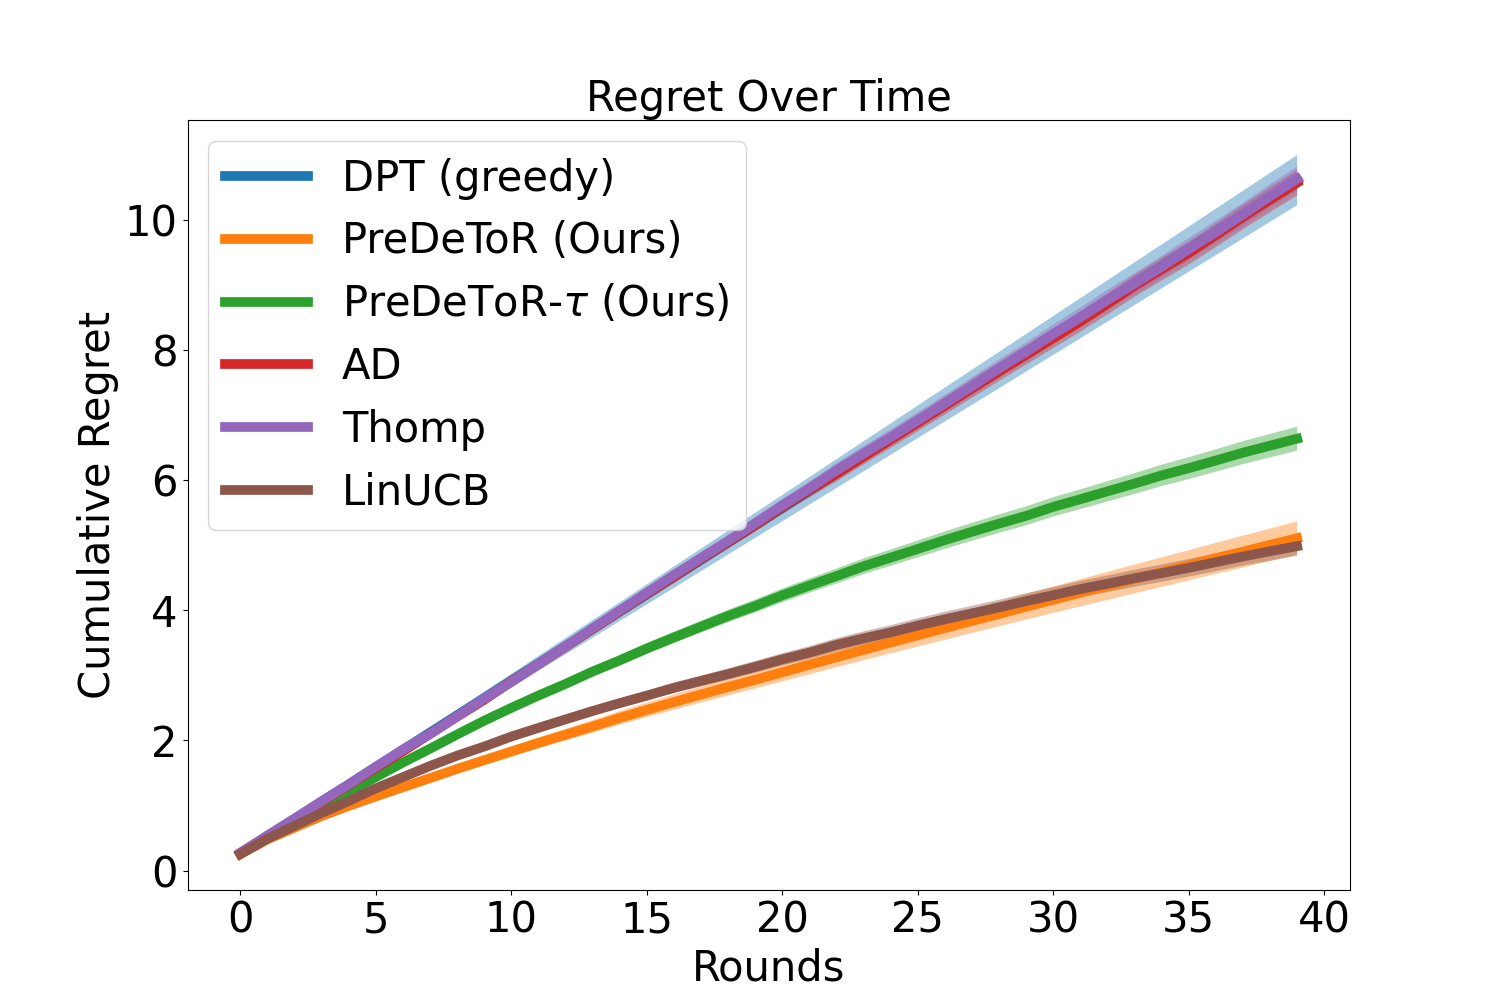
\includegraphics[scale=0.15]{img/Neurips/limit/nlm_lim_lr0.00015_do0_embd32_layer4_head4_envs200195_hists1_samples1_var0.3_cov0.0_H40_d100_lind5_seed1_testcov0.0_hor40.pkl.png}
   \caption{Non-linear Bandit}
   \label{fig:lim-nlm}
\end{subfigure}
\vspace*{-1em}
\caption{Testing the limit experiments. The horizontal axis is the number of rounds. Confidence bars show one standard error.}
\label{fig:expt-lim}
\vspace{-0.7em}
\end{figure}

\textbf{Experimental Result:} We observe these outcomes in \Cref{fig:expt-lim}. In \Cref{fig:lim-lin} we show the linear bandit setting for $\Mpr = 250000$, $\Mts = 200$, $A=100$, $n=50$ and $d=5$. 
%
%
Again, the demonstrator $\pi^w$ is the \ts\ algorithm. We observe that \pred\ (\gt) has lower cumulative regret than \dptg\ and \ad. Note that for any task $m$ the \ts\ will not be able to sample all the actions even once.
% Moreover \pred\ matches the performance of \linucb. 
%
The weak performance of \dptg\ can be attributed to both short horizons and the inability to estimate the optimal action for such a short horizon $n < A$. The \ad\ performs similar to the demonstrator \ts\ because of its training.
%
%Note that for this small horizon setting the \dptg\ does not have a good estimation of $\widehat{a}_{m,*}$ which results in a poor prediction of optimal action $\widehat{a}_{m,t,*}$. 
% This results in higher regret. 
Observe that \pred\ (\gt) has similar regret to \linucb\ and lower regret than \ts\ which also shows that \pred\ is exploiting the latent linear structure of the underlying tasks.
%
In \Cref{fig:lim-nlm} we show the non-linear bandit setting for horizon $n=40$, $\Mpr = 200000$, $A=60$, $d=2$, and $|\Anc|=5$. The demonstrator $\pi^w$ is the \ts\ algorithm.
%
% The training of \ad\ ensures that it does not outperform the demonstrator \ts.
%
Again we observe that \pred\ (\gt) has lower cumulative regret than \dptg, \ad\ and \linucb\ which fails to perform well in this non-linear setting due to its algorithmic design. 

% In the following two experiments, we test the limit of generalization of \pred\ by increasing the number of dimensions. In the linear setting experiment, we use $\Mpr = 400000$, $\Mts = 200$, $d=40$, $A=20$, and $n=15$. In the non-linear setting, we use $\Mpr = 300000$, $\Mts = 200$, $d=15$, $A=30$, and $n=15$. 
% %
% The corresponding results are shown in \Cref{fig:lim-dim-lin} and \Cref{fig:lim-dim-nlm}. Observe that in the non-linear setting, the performance of \pred\ degrades and is almost similar to \dptg. This shows that as the number of dimensions increases and feedback is more complex, the ability of \pred\ to exploit the underlying latent structure and reward correlation also decreases.

